\date{}
\title{}
\date{}
\usepackage{pgfplots}
\pgfplotsset{compat=1.14}
\begin{document}
\begin{frame}
    \titlepage
\end{frame}

\begin{frame}
\frametitle{last time}
    \begin{itemize}
    \item HTTP trailers
    \item cookies
        \begin{itemize}
        \item set-cookie and cookie headers
        \item used for tracking
        \item third-party cookie heuristics
        \end{itemize}
    \item HTTP caching
        \begin{itemize}
        \item headers controlling validity
        \item ability to revalidate
        \end{itemize}
    \item supercookies (cache, sharing connections, etc. as cookies)
        \begin{itemize}
        \item mitigations through separate caches/connections/etc.
        \end{itemize}
    \end{itemize}
\end{frame}

\section{proxies and reverse proxies}
\usetikzlibrary{arrows.meta}
\begin{frame}{HTTP proxies (1)}
\includegraphics[height=0.9\textheight]{../http/moz-proxy-config}
\end{frame}

\begin{frame}
\begin{tikzpicture}
\node[draw, very thick,align=center] (user agent) at (0, 0) {
    user-agent \\ (example: \\ web browser)
};
\node[draw, very thick,align=center] (proxy) at (6, 0) {
    proxy \\server
};
\node[draw, very thick,align=center] (web server) at (12, 0) {
    web \\server
};
\draw[thick,Latex-Latex] (user agent) -- (proxy)
    node[pos=0,above right] {client}
    node[pos=1,above left] {server}
    coordinate[midway] (midpt cp);
\draw[thick,Latex-Latex] (proxy) -- (web server)
    node[pos=0,above right] {client}
    node[pos=1,above left] {server}
    coordinate[midway] (midpt ps);
\draw (midpt cp) -- ++(0cm, -1cm) node[below,align=center] {
    request specifies \\
    which web server \\
    to contact
};
\draw (midpt ps) -- ++(0cm, -1cm) node[below,align=center] {
    looks like normal \\
    user-agent request 
};
\end{tikzpicture}
\end{frame}

\begin{frame}[fragile]{HTTP proxies (2)}
browser$\rightarrow$HTTP(S) proxy sever: \\
\begin{Verbatim}
GET http://example.com/somesite HTTP/1.1
Host: example.com
...
\end{Verbatim}
\rule{.9\textwidth}{1mm}
\begin{itemize}
    \item instead of path, can put full URL
    \item doesn't have to be \texttt{http} URL
\end{itemize}
\end{frame}

\begin{frame}{proxy functionality}
    \begin{itemize}
    \item caching for multiple users
        \begin{itemize}
        \item reason for \texttt{Cache-Control: private}
        \end{itemize}
    \item filtering content
        \begin{itemize}
        \item antimalware, adblocking, etc.
        \end{itemize}
    \item logging content (example: debugging webapp)
    \item \ldots
    \end{itemize}
\end{frame}

\begin{frame}
\begin{tikzpicture}
\node[draw, very thick,align=center] (user agent) at (0, 0) {
    user-agent \\ (example: \\ web browser)
};
\node[draw, very thick,align=center] (proxy) at (6, 0) {
    forward proxy \\server
};
\node[draw, very thick,align=center] (web server) at (12, 0) {
    web \\server
};
\draw[thick,Latex-Latex] (user agent) -- (proxy)
    node[pos=0,above right] {client}
    node[pos=1,above left] {server}
    coordinate[midway] (midpt cp);
\draw[thick,Latex-Latex] (proxy) -- (web server)
    node[pos=0,above right] {client}
    node[pos=1,above left] {server}
    coordinate[midway] (midpt ps);
\draw (midpt cp) -- ++(0cm, -1cm) node[below,align=center] {
    request specifies \\
    which web server \\
    to contact
};
\draw (midpt ps) -- ++(0cm, -1cm) node[below,align=center] {
    looks like normal \\
    user-agent request 
};

\begin{scope}[yshift=-5cm,name prefix=rvs-]
\node[draw, very thick,align=center] (user agent) at (0, 0) {
    user-agent \\ (example: \\ web browser)
};
\node[draw, very thick,align=center] (proxy) at (6, 0) {
    reverse proxy \\server
};
\node[draw, very thick,align=center] (web server) at (12, 0) {
    backend\\server
};
\draw[thick,Latex-Latex] (user agent) -- (proxy)
    node[pos=0,above right] {client}
    node[pos=1,above left] {server}
    coordinate[midway] (midpt cp);
\draw[thick,Latex-Latex] (proxy) -- (web server)
    node[pos=0,above right] {client}
    node[pos=1,above left] {server}
    coordinate[midway] (midpt ps);
\draw (midpt cp) -- ++(0cm, -1cm) node[below,align=center] {
    looks like normal \\
    user-agent request
};
\draw (web server) -- ++(-1cm, -1cm) node[below,align=center] {
    selected from \\
    user-agent request path
};
\end{scope}
\end{tikzpicture}
\end{frame}

\begin{frame}{reverse proxy}
    \begin{itemize}
    \item why not just go directly to actual web server?
    \vspace{.5cm}
    \item make multiple web severs appear as one? example:
        \begin{itemize}
        \item https://example.com/foo/XXX goes to https://foo-backend.example.com/XXX
        \item https://example.com/bar/XXX goes to https://bar-backend.example.com/XXX
        \item https://example.com/ goes to https://frontpage.example.com/
        \end{itemize}
    \item do caching, filtering, or similar on behalf of webservers
    \item split requests between multiple identical servers for performance
    \end{itemize}
\end{frame}

\begin{frame}[fragile]{non-HTTP in HTTP proxy}
\small
client $\rightarrow$ server:
\begin{Verbatim}
CONNECT ns.foo.com:53 HTTP/1.1
Host: ns.foo.com:50
\end{Verbatim}
\rule{.95\textwidth}{1mm} \\
server $\rightarrow$ client:
\begin{Verbatim}
HTTP/1.1 200 OK
Some-header: some-value

\end{Verbatim}
\rule{.95\textwidth}{1mm} \\
client $\rightarrow$ server: (dns request) \\
server $\rightarrow$ client: (dns response from ns.foo.com) \\
client $\rightarrow$ server: (dns request) \\
server $\rightarrow$ client: (dns response from ns.foo.com) \\
\ldots
\end{frame}

\begin{frame}{CONNECT}
    \begin{itemize}
    \item allows ``tunnelling'' arbitrary TCP connections through HTTP
    \item often not implemented by HTTP proxies and/or very restricted
    \end{itemize}
\end{frame}


% FIXME: exercise
    % proxy + reverse proxy
        % which headers, URIs?
        % caching ideas
\subsection{exercise}
\begin{frame}
    \frametitle{proxy exercise}
    \begin{itemize}
    \item suppose we have webapp at running on existing server https://foo.com/
    \item \ldots and it serves images at https://foo.com/images/IMAGENAME
        \begin{itemize}
        \item but it slow at doing so
        \end{itemize}
    \vspace{.5cm}
    \item we want to use faster, caching webserver to server images
    \item if we add a new server to do this, options to configure \\
        both the new and existing server?
        \begin{itemize}
        \item do we need changes to webapp code?
        \item which should be proxies/reverse proxies?
        \end{itemize}
    \end{itemize}
\end{frame}


\subsection{aside: wikimedia architecture}
\begin{frame}{Wikimedia architecture}
\includegraphics[height=0.85\textheight]{../http/Wikipedia_webrequest_2022.png}
\end{frame}


\section{SSO}
\begin{frame}{single-sign on}
\begin{itemize}
\item client $\rightarrow$ foo.com: GET /foo
\item foo.com $\rightarrow$ client: redirect to https://sso.com/login?from=foo.com\&\ldots
\item client $\rightarrow$ sso.com: GET /login?from=foo.com\&\ldots
    \begin{itemize}
    \item sent with cookies set by sso.com
    \end{itemize}
\item sso.com $\rightarrow$ client: web page with form action=http://foo.com/... and method=post
    \begin{itemize}
    \item data in form tells foo.com about username, etc.
    \item cryptographically signed or similar
    \item remember login: possibly script to submit automatically
    \end{itemize}
\item client $\rightarrow$ foo.com: POST /... with data from sso.com
\end{itemize}
\end{frame}

\begin{frame}{single-sign on and third-party cookie awkwardness}
    \begin{itemize}
    \item single-sign on flow also gives a way to do tracking\ldots
    \item not `third-party' cookies since the `root' web page becomes the single-sign on site
    \end{itemize}
\end{frame}



\section{REST}
\begin{frame}{REST}
    \begin{itemize}
    \item REpresentational State Transfer
    \item idea for application interface on top of HTTP
    \vspace{.5cm}
    \item entities in system represented with URLs
    \item GET requests to get state of that entity
    \item PUT and/or POST requests to update entity state
    \item DELETE requests to remove entity
    \end{itemize}
\end{frame}

\begin{frame}[fragile]{example: Canvas API for announcements (1)}
client $\rightarrow$ canvas HTTP server:
\begin{Verbatim}[fontsize=\fontsize{9}{10}\selectfont]
GET /api/v1/announcements?context_codes[]=course_name HTTP/1.1
Authorization: Bearer [secret code]
\end{Verbatim}
\rule{0.9\textwidth}{1mm}
\begin{Verbatim}[fontsize=\fontsize{9}{10}\selectfont]
HTTP/1.1 200 OK
...

[{
  "id": 1,
  "title": "Hear ye",
  "message": "Henceforth, all assignments must be...",
  "posted_at": "2017-01-31T22:00:00Z",
  "delayed_post_at": null,
  "context_code": "course_name",
  ...
},{
 ...
]
\end{Verbatim}
\end{frame}



\subsection{REST exercise}
\begin{frame}
\frametitle{REST exercise}
\begin{itemize}
\item suppose I want a REST-like interface to book train tickets
\item what should that look like?
    \begin{itemize}
    \item type of request to book new tickets?
    \item to modify? to cancel?
    \item to lookup all tickets booked on train? by one user?
    \end{itemize}
\end{itemize}
\end{frame}


\section{multiaccess media}

% multiple channels?
    % everyone receives everything?
% start with simple model
\begin{frame}{multiaccess media}
    \begin{itemize}
    \item shared air for radio/light signals
    \item shared wires for electrical/light signals
    \item \ldots
    \vspace{.5cm}
    \item needs:
        \begin{itemize}
        \item way to tell what signals are for whom
        \item way to decide who `talks' when/where
        \end{itemize}
    \end{itemize}
\end{frame}

\begin{frame}{shared wires}
    \begin{itemize}
    \item used to be how Ethernet worked
        \begin{itemize}
        \item before Ethernet switches were ubiquitous
        \end{itemize}
    \item how cable Internet works
        \begin{itemize}
        \item shared line to many customers in area
        \item need to share
        \end{itemize}
    \item usually how fiber-to-the-home works
        \begin{itemize}
        \item ``passive optical network''
        \item connect multiple fibers optically
        \end{itemize}
    \end{itemize}
\end{frame}

\begin{frame}{multiple channels}
    \begin{itemize}
    \item can have multiple channels over single medium
    \item typically: radio or electrical signal or light frequencies
    \item sender/receiver separate channels electrically/optically
    \vspace{.5cm}
    \item to start: will worry about coordinating one chnanel
    \end{itemize}
\end{frame}

\begin{frame}{wireless spectrum}
    \begin{itemize}
    \item most useful radio spectrum \textit{licensed}
    \item gov't gives exclusive rights (within some region) to specific organizations/poeple 
        \begin{itemize}
        \item example: cellular, TV, satellite, air traffic control, etc.
        \end{itemize}
    \item a lot of computer networking uses \textit{unlicensed} bands
        \begin{itemize}
        \item use without specific permission allowed
        \item still limits on power, procedures to avoid interference
        \end{itemize}
    \end{itemize}
\end{frame}

\begin{frame}{selected unlicensed bands}
    \begin{itemize}
    \item approx. frequencies unlicensed in US (not everywhere)
    \vspace{.5cm}
    \item 902--928 MHz (802.15.4 (IoT focused))
    \item 2.4--2.5 GHz (802.15.4; 802.11b/g/n/ax/\ldots; bluetooth; microwave ovens)
    \item 5.15 GHz--5.25 GHz (802.11a/n/ac/ax/\ldots)
    \item 5.25 GHz--5.73 GHz (802.11a/n/ac/ax/\ldots; also weather radar)
        \begin{itemize}
        \item requires `dynamic frequency selection'
        \end{itemize}
    \item 5.73 GHz--5.85 GHz (802.11a/n/ac/ax/\ldots)
    \item 5.93 GHz--7.12 GHz (802.11ax/\ldots)
    \item 24.0-24.2 GHz
    \item 57--64 GHz
    \end{itemize}
\end{frame}



\subsection{collisions}
\begin{frame}{collisions}
    \begin{itemize}
    \item $N$ nodes try to transmit one channel at same time
    \item likely outcomes for some receiver:
    \vspace{.5cm}
    \item receiver gets garbage
        \begin{itemize}
        \item ``collision''
        \end{itemize}
    \item receiver receives 1 of the $N$ collisions
    \end{itemize}
\end{frame}



\section{transmitting in the blind}
% FIXME: exercise: maximum transmission rate if \ldots
\usetikzlibrary{arrows.meta}
\begin{frame}{running example}
\begin{itemize}
    \item based on Abramson, ``The Aloha System---Another alternative for computer comunications'' (1970)
    \vspace{.5cm}
    \item suppose we have shared radio with nodes A1, A2, \ldots, A$n$ and B
    \vspace{.5cm}
    \item A1, A2, \ldots A$n$ are all trying to transmit to B
    \item takes 1 ms to send message
    \item and want to collectively send $k$ messages per second
        \begin{itemize}
        \item randomly spaced (exponential distribution)
        \end{itemize}
\end{itemize}
\end{frame}

\begin{frame}{some probability}
    \begin{itemize}
    \item exponential distribution with mean $\lambda$
        \begin{itemize}
        \item our model for when packets sent
        \item ``memoryless'' distribution
        \item knowing when last packet sent tells you nothing about next
        \item (yes, not realistic)
        \end{itemize}
    \vspace{.5cm}
    \item probability events occur $< K$ time units apart \\
    $1-e^{-\lambda K}$
    \end{itemize}
\end{frame}


\begin{frame}{quiet time to avoid collisions}
\begin{tikzpicture}
\begin{scope}[x=3cm]
    \draw[line width=1mm,-Latex] (-0.5, 0) -- (4, 0) node[above,midway] {time};
    \draw[thick,fill=violet] (1.5, -0.5) rectangle ++(1, -1);
    \draw[thick,fill=violet,opacity=0.5] (0.55, -2) rectangle ++(1, -1);
    \draw[thick,fill=violet,opacity=0.5] (2.45, -2) rectangle ++(1, -1);
    \path[fill=red!60!black] (0.5,-1.7) rectangle ++(2, -.2);
    \path[fill=green] (-0.5,-1.7) rectangle ++(1, -.2);
    \path[overlay,fill=green] (2.5,-1.7) rectangle ++(2, -.2);
    \draw[dotted,very thick] (1.5, -3) -- (1.5, -0.5);
    \draw[dotted,very thick] (2.5, -3) -- (2.5, -0.5);
\end{scope}
\end{tikzpicture}
\begin{itemize}
\item to avoid collision with 1 ms packet\ldots
\item can't start packet less than 1 ms before
\item can't start packet less than 1 ms after
\item $\rightarrow$ need 2 ms without other packet starting for no collision
\end{itemize}
\end{frame}
% FIXME: diagram of 1.5 ms apart starts and collision

\begin{frame}{chance of collisions?(1)}
    \begin{itemize}
    \item to avoid collision when sending 1 ms packet
    \item need no other packet to be sent in 2ms period around its start time
    \vspace{.5cm}
    \item with $k$ packets/sec, chance is approx $1-e^{-\frac{2}{1000}k}$
    \end{itemize}
\end{frame}

\begin{frame}{chance of collision}
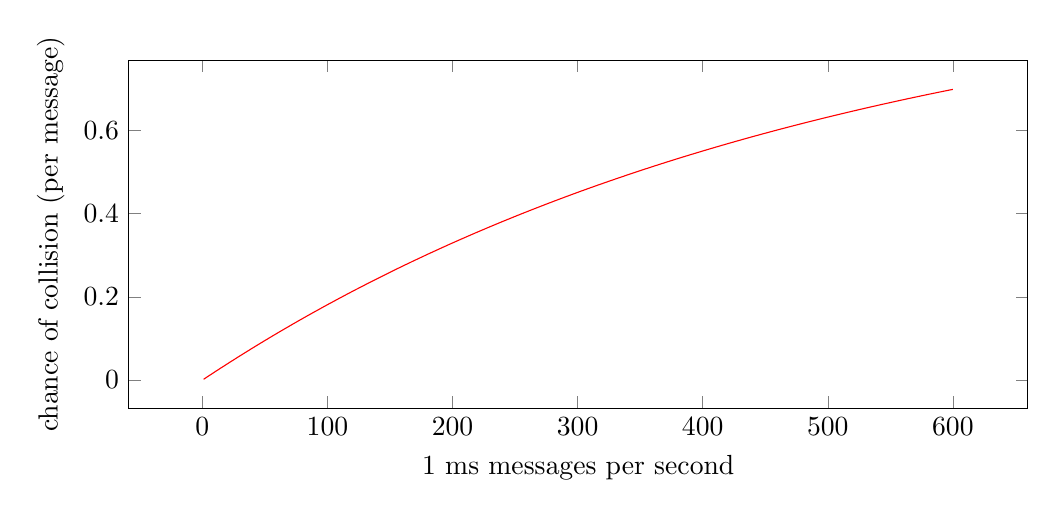
\begin{tikzpicture}
\begin{axis}[xlabel=1 ms messages per second,ylabel=chance of collision (per message),width=13cm,height=6cm]
\addplot[domain=1:600,color=red,samples=1000]{1-exp(-(2 * x)/1000};
\end{axis}
\end{tikzpicture}
\end{frame}

\begin{frame}{retransmissions}
    \begin{itemize}
    \item what's going to happen when node can't send message
    \item probably it will retransmit it\ldots
    \vspace{.5cm}
    \item which means real transmission rate will be some $R > k$
        \begin{itemize}
        \item where $k$ is rate messages are generated
        \end{itemize}
    \item about $[1-e^{-2R\frac{1}{1000}}]$ chance of each message generated
    \item so $R = k + \left(1-e^{-2R\frac{1}{1000}}\right) \cdot R$
    \item $R = k + R - Re^{-2R\frac{1}{1000}}$
    \item $k = Re^{-2R\frac{1}{1000}}$
    \end{itemize}
\end{frame}

\begin{frame}{retransmissions (plot)}
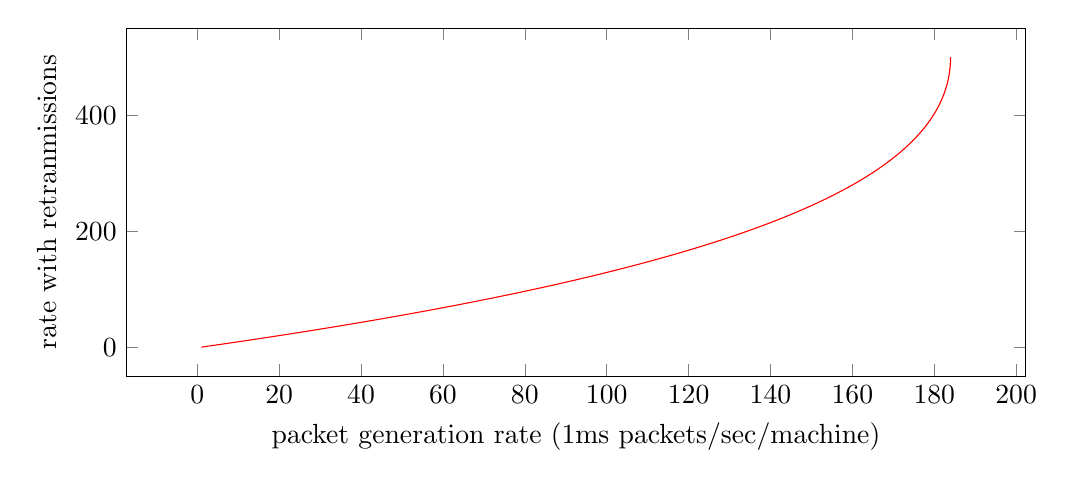
\begin{tikzpicture}
\begin{axis}[xlabel={packet generation rate (1ms packets/sec/machine)}, ylabel={rate with retranmissions},width=13cm,height=6cm]
\addplot[domain=1:500,color=red,samples=1000] (x * exp(-2*x/1000), x);
\end{axis}
\end{tikzpicture}
\end{frame}



\begin{frame}{thinking about result}
    \begin{itemize}
    \item sending 500 1ms packet or retransmission/second
        \begin{itemize}
        \item using about half the capacity!
        \end{itemize}
    \item representing $\sim$ 186 1 ms non-retranmissions/second
        \begin{itemize}
        \item $\frac{1}{2e} = 0.186\ldots$
        \item using about 1/6th the capacity
        \end{itemize}
    \vspace{.5cm}
    \item results hold generally
    \item seems pretty bad for shared channel efficiency!
    \end{itemize}
\end{frame}

\begin{frame}
\frametitle{some assumptions we made}
    \begin{itemize}
    \item exponential model assumes transmission time of message X doesn't affect transmission time of message Y
    \vspace{.5cm}
    \item if node A has messages A1, A2 to transmit, it won't start transmitting A2 until after A1 done
        \begin{itemize}
        \item means this model is probably pessimistic with only a few transmitters
        \end{itemize}
    \item assumes nodes won't look at prior other transmissions to decide when to transmit
    \end{itemize}
\end{frame}



\section{carrier-sense multiple access}
\usetikzlibrary{arrows.meta}
\begin{frame}{carrier sense}
    \begin{itemize}
    \item channel can be `busy' or not
    \item radio/light:
        \begin{itemize}
        \item have some sort of signal detectable on frequency
        \end{itemize}
    \vspace{.5cm}
    \item ``carrier sense''
    \item way to detect whether channel busy
    \end{itemize}
\end{frame}

\begin{frame}{using carrier sense}
    \begin{itemize}
    \item simple idea: don't transmit if channel already busy
    \vspace{.5cm}
    \item problem: then when do you transmit?
    \item some options:
        \begin{itemize}
        \item never, lose the packet
        \item immediately when it stops being busy
        \item sometime after it stops being busy
        \end{itemize}
    \end{itemize}
\end{frame}

\begin{frame}{`slots'}
\begin{itemize}
\item if packets take a fixed amount of time\ldots
\item want to wait whole number of packet times
    \begin{itemize}
    \item immediately after, one after, two after, three after
    \end{itemize}
\item avoids requiring almost 2 packets worth of `quiet' time
\item can synchronize by observing end of last transmission
\end{itemize}
\begin{tikzpicture}
\begin{scope}[x=3cm]
    \draw[line width=1mm,-Latex] (-0.5, 0) -- (4, 0) node[above,midway] {time};
    \draw[thick,fill=violet] (0.0, -0.5) rectangle ++(1, -1);
    \foreach \x in {1,2,3} {
        \draw[dotted,line width=0.7mm] (\x, -0.25) -- ++ (0, -2);
    }
\end{scope}
\end{tikzpicture}
\end{frame}

\begin{frame}{802.11b typical slots}
    \begin{itemize}
    \item $20 \mu\text{s}$ slots
    \item $50 \mu\text{s}$ interframe spacing (IFS)
        \begin{itemize}
        \item includes time to receive ACK of packet
        \end{itemize}
    \vspace{.5cm}
    \item transmit first time after IFS (if idle)
    \item transmit second time after IFS + rand($0$, $2^5$) slots
        \begin{itemize}
        \item plus time spent by other seen transmissions
        \end{itemize}
    \item third time after rand($0$, $2^6$) slots, etc.
    \end{itemize}
\end{frame}


\subsection{collision detection versus avoidance}
    % FIXME: diagram for ethernet collision detection + retransmit
\begin{frame}{collision detection}
    \begin{itemize}
    \item Wi-Fi: use ACKs to detect if transmission successful
    \item problem: transmit whole packet, then know about collision
    \vspace{.5cm}
    \item alternate idea: listen for collision, stop transmitting early
    \item doesn't work on wireless (we'll talk about why later)
    \item but does work on some wired shared media
    \item part of reason for design of Ethernet header
    \end{itemize}
\end{frame}

\usetikzlibrary{arrows.meta,shapes,shapes.misc}
\begin{frame}{collision detection takes time}
\begin{tikzpicture}[y=0.7cm]
\tikzset{
    wire/.style={draw,very thick,Circle-Circle},
    signal1/.style={draw,line width=1mm,red,-Latex},
    signal2/.style={draw,line width=2mm,dotted,violet,-Latex},
}
\draw[wire] (0, 0) -- (12, 0);
\draw[wire] (0, -1) -- (12, -1);
\draw[signal1] (0, -1) -- (2, -1);

\draw[wire] (0, -2) -- (12, -2);
\draw[signal1] (0, -2) -- (4, -2);
\draw[signal2] (12, -2) -- (10, -2);

\draw[wire] (0, -3) -- (12, -3);
\draw[signal1] (0, -3) -- (6, -3);
\draw[signal2] (12, -3) -- (8, -3);

\draw[wire] (0, -4) -- (12, -4);
\draw[signal1] (0, -4) -- (8, -4);
\draw[signal2] (12, -4) -- (6, -4);

\draw[wire] (0, -5) -- (12, -5);
\draw[signal1] (0, -5) -- (10, -5);
\draw[signal2] (12, -5) -- (4, -5);

\draw[wire] (0, -6) -- (12, -6);
\draw[signal1] (0, -6) -- (12, -6);
\draw[signal2] (12, -6) -- (2, -6);
\node[draw=red,line width=2mm,minimum width=.5cm,minimum height=.5cm,cross out] at (13, -6) {};

\draw[wire] (0, -7) -- (12, -7);
\draw[signal1] (0, -7) -- (12, -7);
\draw[signal2] (11, -7) -- (0, -7);
\node[draw=red,line width=2mm,minimum width=.5cm,minimum height=.5cm,cross out] at (-1, -7) {};

\draw[wire] (0, -8) -- (12, -8);
\draw[signal1] (2, -8) -- (12, -8);
\draw[signal2] (9, -8) -- (0, -8);
\end{tikzpicture}
\end{frame}


\section{wireless model, hidden and exposed nodes} 
\begin{frame}{free space wireless transmission}
\begin{itemize}
\item assuming 2.4GHz Wifi, no obstacles, omnidirectional transmission:
\item 10 dB loss = $\frac{1}{10}$th power; 20 dB loss = $\frac{1}{100}$th power
\end{itemize}
\begin{tikzpicture}
\begin{axis}[
    xlabel={distance from transmitter (m)},
    ylabel={lost signal (dB)}
]
\addplot table {freespacemodel.table};
%\addplot[domain=0.1:100,samples=100] { 20*log(d/1000.0)/log(10) + 20*log(2.4)/log(10) + 92.45 };
\end{axis}
\end{tikzpicture}
\end{frame}

\begin{frame}{multipath interference}
\end{frame}


\section{RTS/CTS}

\begin{frame}{ready-to-send/clear-to-send}
    \begin{itemize}
    \item can't detect likely interference at sender
    \item but can at receiver
    \vspace{.5cm}
    \item idea: have receiver tell when it's okay to transmit
    \end{itemize}
\end{frame}


\section{multipath}

\begin{frame}{multipath interference}
\begin{tikzpicture}
\begin{pgfonlayer}{fg}
    \draw[fill=black] (0, 0) circle (.2cm);
    \draw[fill=black] (12, -4) circle (.2cm);
    \begin{scope}[ultra thick]
        \draw (-2, 2) rectangle (13, -5);
    \end{scope}
\end{pgfonlayer}
\tikzset{
    signal/.style={draw,violet,line width=.8mm,-Latex},
    signal fade/.style={draw,violet!60!white,line width=.8mm},
    signal fade2/.style={draw,violet!30!white,line width=.8mm},
    signal end/.style={-{Latex[sep=0.2cm]}},
}
\draw[signal] (0, 0) -- (12 / 3, 6 / 3);
\draw[signal fade,signal end] (12 / 3, 6 / 3) -- (12, -4);
\draw[signal] (0, 0) -- (-14 / 7, -4 / 7);
\draw[signal fade,signal end] (-14 / 7, -4 / 7) -- (12, -4);
\draw[signal] (0, 0) -- (14 * 13 / 14, -4 * 13 / 14);
\draw[signal fade, signal end] (14 * 13 / 14, -4 * 13 / 14) -- (12, -4);
\draw[signal] (0, 0) -- (14 * 5 / 6, -6 * 5 / 6);
\draw[signal fade, signal end] (14 * 5 / 6, -6 * 5 / 6) -- (12, -4);

\draw[signal,signal end] (0, 0) -- (12, -4);
\end{tikzpicture}
\end{frame}

\begin{frame}{simple self-interference}
\begin{tikzpicture}
\begin{axis}[name=top1,hide axis,width=7cm,height=4cm,ymin=-1,ymax=1]
    \addplot[domain=0:1000,samples=1000] {sin(x*4) * sin(0.75+x/3)};
    \coordinate (top1 tl) at (axis cs:0, 1);
    \coordinate (top1 br) at (axis cs:1000, -1);
\end{axis}
\coordinate (middle base) at ([yshift=-2cm]top1.east);
\coordinate (low base) at ([yshift=-4cm]top1.east);
\begin{axis}[anchor=east,name=middle1,at={(middle base)},width=7cm,height=4cm,hide axis,
    ymin=-2,ymax=2]
    \addplot[domain=0:1000,samples=1000] {0.4*(sin((x+45)*4) * sin(0.75+(x + 45)/3))};
    \coordinate (middle1 tl) at (axis cs:0, 1);
    \coordinate (middle1 br) at (axis cs:1000, -1);
\end{axis}
\begin{axis}[hide axis,width=7cm,height=4cm,anchor=east,name=combine1,at={(low base)},
    ymin=-1,ymax=1]
    \addplot[domain=0:1000,samples=1000] {
     sin(x*4) * sin(0.75+x/3) +
     0.5*(sin((x+45)*4) * sin(0.75+(x + 45)/3))
    };
\end{axis}
\coordinate (top2 base) at ([xshift=2cm]top1.east);
\begin{axis}[anchor=west,at={(top2 base)},name=top2,hide axis,width=7cm,height=4cm,ymin=-1,ymax=1]
    \addplot[domain=0:1000,samples=1000] {sin(x*4) * sin(0.75+x/3)};
    \coordinate (top2 tl) at (axis cs:0, 1);
    \coordinate (top2 br) at (axis cs:1000, -1);
\end{axis}
\coordinate (middle base2) at ([yshift=-2cm]top2.east);
\coordinate (low base2) at ([yshift=-4cm]top2.east);
\begin{axis}[anchor=east,name=middle2,at={(middle base2)},width=7cm,height=4cm,hide axis,
    ymin=-1,ymax=1]
    \addplot[domain=0:1000,samples=1000] {0.4*(sin((x+25)*4) * sin(0.75+(x + 45)/3))};
    \coordinate (middle2 tl) at (axis cs:0, 1);
    \coordinate (middle2 br) at (axis cs:1000, -1);
\end{axis}
\begin{axis}[hide axis,width=7cm,height=4cm,anchor=east,name=combine2,at={(low base2)},
    ymin=-1,ymax=1]
    \addplot[domain=0:1000,samples=1000] {
     sin(x*4) * sin(0.75+x/3) +
     0.5*(sin((x+25)*4) * sin(0.75+(x + 25)/3))
    };
\end{axis}
\node[font=\large]  at (middle1.west) {+};
\node[font=\large]  at (middle2.west) {+};
\draw[ultra thick] (middle1.south west) -- (middle1.south east);
\draw[ultra thick] (middle2.south west) -- (middle2.south east);
\begin{visibleenv}<2>
\draw[red] (top1 tl) rectangle (top1 br);
\node[font=\small,anchor=west,red] at (top1.east) {original};
\draw[blue] (middle1 tl) rectangle (middle1 br);
\node[font=\small,anchor=west,blue] at (middle1.east) {reflected};
\end{visibleenv}
\end{tikzpicture}
\end{frame}

\begin{frame}{multipath interference}
    \begin{itemize}
    \item quite complicated to predict in three dimensions, variable reflectivity, \ldots
    \item can help and hurt signal reception
    \end{itemize}
\end{frame}




\subsection{hidden terminals, exposed nodes}

% FIXME: short interframe spacing

\section{aside: assignment}

\subsection{RTS/CTS}

\subsection{polling mode}

\section{ad-hoc versus base station}

\subsection{probes and associations}

\subsection{mobility}

\subsection{channels}

\section{time-division multiple access}

\section{frequency/carrier-divison multiple access}



\section{backup slides}
\begin{frame}\frametitle{backup slides}
\end{frame}

\section{supercookies}
\input{../http/cache-as-cookies}


\end{document}
